\documentclass[11pt, a4paper]{article}\usepackage[]{graphicx}\usepackage[]{color}
%% maxwidth is the original width if it is less than linewidth
%% otherwise use linewidth (to make sure the graphics do not exceed the margin)
\makeatletter
\def\maxwidth{ %
  \ifdim\Gin@nat@width>\linewidth
    \linewidth
  \else
    \Gin@nat@width
  \fi
}
\makeatother

\definecolor{fgcolor}{rgb}{0.345, 0.345, 0.345}
\newcommand{\hlnum}[1]{\textcolor[rgb]{0.686,0.059,0.569}{#1}}%
\newcommand{\hlstr}[1]{\textcolor[rgb]{0.192,0.494,0.8}{#1}}%
\newcommand{\hlcom}[1]{\textcolor[rgb]{0.678,0.584,0.686}{\textit{#1}}}%
\newcommand{\hlopt}[1]{\textcolor[rgb]{0,0,0}{#1}}%
\newcommand{\hlstd}[1]{\textcolor[rgb]{0.345,0.345,0.345}{#1}}%
\newcommand{\hlkwa}[1]{\textcolor[rgb]{0.161,0.373,0.58}{\textbf{#1}}}%
\newcommand{\hlkwb}[1]{\textcolor[rgb]{0.69,0.353,0.396}{#1}}%
\newcommand{\hlkwc}[1]{\textcolor[rgb]{0.333,0.667,0.333}{#1}}%
\newcommand{\hlkwd}[1]{\textcolor[rgb]{0.737,0.353,0.396}{\textbf{#1}}}%
\let\hlipl\hlkwb

\usepackage{framed}
\makeatletter
\newenvironment{kframe}{%
 \def\at@end@of@kframe{}%
 \ifinner\ifhmode%
  \def\at@end@of@kframe{\end{minipage}}%
  \begin{minipage}{\columnwidth}%
 \fi\fi%
 \def\FrameCommand##1{\hskip\@totalleftmargin \hskip-\fboxsep
 \colorbox{shadecolor}{##1}\hskip-\fboxsep
     % There is no \\@totalrightmargin, so:
     \hskip-\linewidth \hskip-\@totalleftmargin \hskip\columnwidth}%
 \MakeFramed {\advance\hsize-\width
   \@totalleftmargin\z@ \linewidth\hsize
   \@setminipage}}%
 {\par\unskip\endMakeFramed%
 \at@end@of@kframe}
\makeatother

\definecolor{shadecolor}{rgb}{.97, .97, .97}
\definecolor{messagecolor}{rgb}{0, 0, 0}
\definecolor{warningcolor}{rgb}{1, 0, 1}
\definecolor{errorcolor}{rgb}{1, 0, 0}
\newenvironment{knitrout}{}{} % an empty environment to be redefined in TeX

\usepackage{alltt}
\usepackage{cmap}                
\usepackage[T2A]{fontenc}
\usepackage[utf8]{inputenc}
\usepackage{mathtext}
\usepackage[english,russian]{babel}
\usepackage{commath}
\usepackage{amsfonts}
\usepackage{amssymb}
\usepackage{amsmath}
\usepackage{amsthm}
\usepackage{mathtools}
\usepackage{indentfirst}
\usepackage{geometry}
\usepackage{tikz}
\usepackage{spalign}
\usepackage{tkz-euclide}
\usepackage{soul}
\usetkzobj{all}
\usetikzlibrary{arrows,positioning}
\usetikzlibrary{shapes,snakes}
\usetikzlibrary{shapes.multipart}
\usepackage{graphicx}
\usepackage{epstopdf}
\usepackage{subcaption}
\usepackage{caption}
\usepackage{hyperref}
\usepackage{setspace}
\usepackage{float}
\usepackage{tcolorbox}
\usepackage{amsmath}
\usepackage{physics}
\captionsetup{justification=centering}
\DeclareMathOperator*{\argmin}{argmin}
\DeclareMathOperator*{\argmax}{argmax}
\providecommand{\TODO}{\fcolorbox{red}{red}{\large{TODO}}}
\DeclareMathOperator{\upd}{upd}
\DeclareMathOperator{\eol}{eol}
\DeclarePairedDelimiter\ceil{\lceil}{\rceil}
\DeclarePairedDelimiter\floor{\lfloor}{\rfloor}
\providecommand{\err}[1]{$\mathcal{#1}$}
\providecommand{\ev}[1]{$\mathbb{#1}$}
\providecommand{\TODO}[1]{\fcolorbox{red}{red}{\large{FIxME}:#1}}
\providecommand{\PRACTICE}{\fcolorbox{blue}{blue}{\large{PRACTICE}}}
\usepackage{physics}
\DeclareMathOperator{\sign}{sign}
\makeatletter
\newenvironment{sqcases}{%
  \matrix@check\sqcases\env@sqcases
}{%
  \endarray\right.%
}
\def\env@sqcases{%
  \let\@ifnextchar\new@ifnextchar
  \left\lbrack
  \def\arraystretch{1.2}%
  \array{@{}l@{\quad}l@{}}%
}
\newenvironment{ecases}{%
  \matrix@check\ecases\env@ecases
}{%
  \endarray\right.%
}
\def\env@ecases{%
  \let\@ifnextchar\new@ifnextchar
  \left.
  \def\arraystretch{1.2}%
  \array{@{}l@{\quad}l@{}}%
}
%% for inline R code: if the inline code is not correctly parsed, you will see a message
\newcommand{\rinline}[1]{SOMETHING WRONG WITH knitr}


\title{Support Vector Machines}
\author{Д.\,Корчемкин, В.\,Агеев\,\\622 группа}
\IfFileExists{upquote.sty}{\usepackage{upquote}}{}
\begin{document}
\maketitle 

\section{SVM}
Будем рассматривать задачу классификации в рамках обучения с учителем.

Имеется выборка $\left\{\left(x_1, y_1\right), \dots, \left(x_n, y_n\right)\right\}$, $x_i\in\mathbb{R}^p$, $y_i\in\left\{-1, 1\right\}$;
задачей является построение классифицирующего правила $f:\mathbb{R}^p\rightarrow \left\{-1, 1\right\}$.

Отметим, что никаких дополнительных ограничений на распределение не требуется.

\subsection{Hard-margin SVM\label{sec:hm}}
Предположим, что присутсвует линейная разделимость, т.е. существует гиперплоскость (определяемая уравнением $x^\intercal \beta-\beta_0=0$ ($x,\beta\in\mathbb{R}^p; \beta_0\in\mathbb{R}$),
такая, что точки, соответствующие разным классам лежат в различных полупространствах относительно гиперплоскости.

Факт принадлежности наблюдений из разных классов разным полупространствам можно (возможно, изменив знаки $\beta, \beta_0$)
описать уравнениями:
\[
\begin{sqcases}
	x_i^\intercal \beta - \beta_0 < 0 & y_i=-1 \\
	x_i^\intercal \beta - \beta_0 > 0 & y_i=1 \\
\end{sqcases}
\Leftrightarrow
\left(x_i^\intercal \beta - \beta_0\right) y_i > 0
\]
В таком случае, классифицирующим правилом разумно принять
\[
g\left(x\right)=\sign{\left(x^\intercal \beta-\beta_0\right)}
\]

Ясно, что в случае линейно разделимых данных может существовать более одной гиперплоскости, разделяющей данные.
Введём критерий оптимальности: максимальное расстояние между двумя гиперплоскостями, параллельных данной и 
симметрично расположенных относительно неё, при котором между ними не находится ни одна из точек $x_i$;
это расстояние будем называть зазором (margin).


Легко видеть, что каждой из двух параллельных гиперплоскостей будет принадлежать некоторое количество
точек из соответствующего класса (иначе, так как количество точек в выборке конечно, то растояние между
гиперплоскостями можно увеличить, сместив гиперплоскость, которой не принадлежит ни одной точки);
точки, которые принадлежат одной из гиперплоскостей --- будем называть опорными векторами.

С точностью до нормировки вектора $\beta$ эта пара гиперплоскостей может быть описана парой уравнений:
\[
\begin{ecases}
	x^\intercal \beta - \beta_0 = -1 \\
	x^\intercal \beta - \beta_0 = 1 \\
\end{ecases}
\]
а растояние между ними составит $\frac{2}{\norm{\beta}}$ (см. поясняющий рисунок \ref{fig:hm}).

\begin{figure}
	\centering
	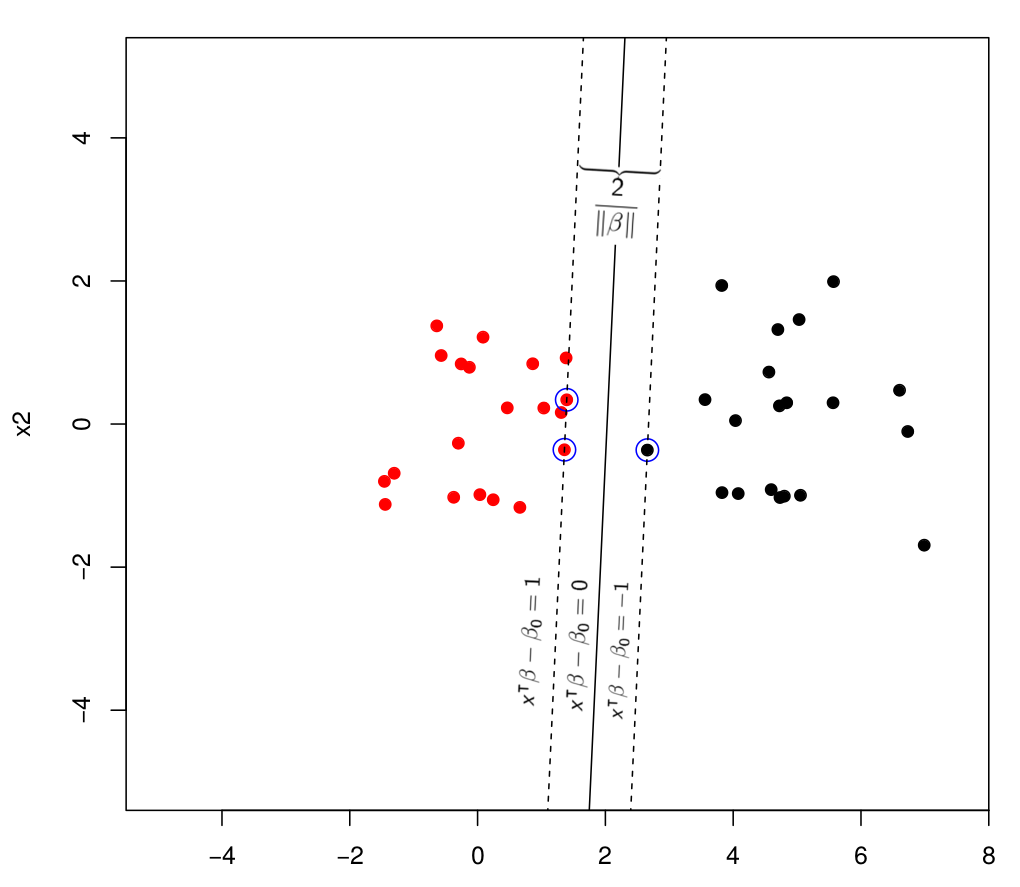
\includegraphics[width=0.7\textwidth]{plot.png}
	\caption{Hard-margin SVM\label{fig:hm}}
\end{figure}

Принадлежность точек обучающей выборки полупространствам описывается уравнениями
\[
\begin{sqcases}
	x_i^\intercal \beta - \beta_0 \leq 1 & y_i=-1 \\
	x_i^\intercal \beta - \beta_0 \geq 1 & y_i=1 \\
\end{sqcases}
\Leftrightarrow
\left(x_i^\intercal \beta - \beta_0\right) y_i \geq 1
\]

Таким образом, в случае линейно разделимой выборки, задача выбора оптимальной гиперплоскости сводится к следующей
задаче квадратичного программирования с линейными ограничениями:
\begin{equation}
\begin{cases}
\frac{1}{2}\norm{\beta}^2_2\rightarrow \min\limits_{\beta, \beta_0} \\
\left(x_i^\intercal \beta - \beta_0\right) y_i \geq 1, \forall i\\
\end{cases}
\label{eq:hard-primal}
\end{equation}

Пользуясь принципом Лагранжа, из \eqref{eq:hard-primal} получаем задачу:
\begin{equation}
\begin{cases}
\inf\limits_{\beta,\beta_0} \frac{1}{2}\norm{\beta}_2^2-\sum\limits_{i=1}^n{\alpha_i\left(y_i\left(x_i^\intercal \beta - \beta_0\right) - 1\right)} \rightarrow \max\limits_{\alpha_1,\dots,\alpha_n} \\
\alpha_i \geq 0, \forall i \\
\end{cases}
\label{eq:hard-dual}
\end{equation}

Так как все функции гладкие, то $\inf$ достигается в точке, в которой выполнены необходимые условия экстремума:
\[
\begin{ecases}
\frac{\partial}{\partial \beta}: & \beta = \sum\limits_{i=1}^{n}\alpha_i y_i x_i \\
\frac{\partial}{\partial \beta_0}: & 0=\sum\limits_{i=1}^{n}\alpha_i y_i \\
\end{ecases}
\]
подставляя эти равенства в \eqref{eq:hard-dual} получаем:
\begin{equation}
\begin{cases}
\sum\limits_{i=1}^n \alpha_i -\frac{1}{2}\sum\limits_{i=1}^{n}\sum\limits_{k=1}^{n}\alpha_i\alpha_k y_i y_k x_i^\intercal x_k \rightarrow \max\limits_{\alpha_1,\dots,\alpha_n} \\
\alpha_i \geq 0, \forall i \\
\sum\limits_{i=1}^{n}\alpha_i y_i=0 \\
\alpha_i \left(y_i\left(x_i^\intercal \beta - \beta_0\right)-1\right) = 0 \\
\end{cases}
\end{equation}

Из условия регулярности ККТ:
\begin{equation}
\alpha_i \left(y_i\left(x_i^\intercal \beta - \beta_0\right)-1\right) = 0 \\
\label{eq:hard-kkt}
\end{equation}
в оптимальной точке, т.е. либо $\alpha_i=0$, либо $x_i$ является опорным вектором (принадлежит одной из пары плоскостей, описаных выше).

Таким образом, решающее правило строится на основе <<сложных>> для классификации наблюдений, а остальные наблюдения --- не влияют (явным образом)
на расположение разделяющей гиперплоскости.

\subsection{Soft-margin SVM\label{sec:sm}}
Понятно, что требование линейной разделимости классов слишком сильное для реальной применимости SVM как метода классификации.

Позволим для этого каждому из ограничений в задаче \eqref{eq:hard-primal} быть несколько ослабленным:
\begin{equation}
\begin{cases}
\frac{1}{2}\norm{\beta}^2_2\rightarrow \min\limits_{\beta, \beta_0} \\
\left(x_i^\intercal \beta - \beta_0\right) y_i \geq 1 - \xi_i, \forall i\\
\sum\limits_{i=1}^{n}\xi_i \leq t \\
\xi_i\geq 0\, \forall i \\
\end{cases}
\label{eq:soft-primal}
\end{equation}
($t$ --- параметр алгоритма; линейно-разделимый случай соответствует $t=0$).

Далее, повторяя все рассуждения для линейно-разделимого случая, используем принцип Лагранжа:
\begin{equation}
\begin{cases}
\inf\limits_{\beta,\beta_0,\xi_1,\dots,\xi_n} \frac{1}{2}\norm{\beta}_2^2+\lambda\sum\limits_{i=1}^{n}\xi_i-\sum\limits_{i=1}^n{\alpha_i\left(y_i\left(x_i^\intercal \beta - \beta_0\right) - \left(1-\xi_i\right)\right)}-\sum\limits_{i=1}^n\gamma_i\xi_i \rightarrow \max\limits_{\alpha_1,\dots,\alpha_n, \gamma_1,\dots,\gamma_n,\lambda} \\
0 \leq \alpha_i \leq t, \forall i \\
\gamma_i \geq 0, \forall i \\
\lambda \geq 0 \\
\end{cases}
\label{eq:soft-dual}
\end{equation}

Опять же, ввиду гладкости, $\inf$ достигается в точке, в которой выполнены необходимые условия экстремума:
\[
\begin{ecases}
\frac{\partial}{\partial \beta}: & \beta = \sum\limits_{i=1}^{n}\alpha_i y_i x_i \\
\frac{\partial}{\partial \beta_0}: & 0=\sum\limits_{i=1}^{n}\alpha_i y_i \\
\frac{\partial}{\partial \xi_i}: & \alpha_i=\lambda-\gamma_i \\
\end{ecases}
\]
используя эти равенства в \eqref{eq:soft-dual}, получаем:
\begin{equation}
\begin{cases}
\sum\limits_{i=1}^n\alpha_i-\frac{1}{2}\sum\limits_{i=1}^{n}\sum\limits_{k=1}^{n}\alpha_i\alpha_ky_iy_kx_i^\intercal x_k \rightarrow \max\limits_{\alpha_1,\dots,\alpha_n} \\
0 \leq \alpha_i \leq t, \forall i \\
\sum\limits_{i=1}^{n}\alpha_i y_i=0 \\
\end{cases}
\label{eq:soft-final}
\end{equation}

Из условия регулярности ККТ опять же следует классификация векторов на опорные, аутлаеры и не участвующие в построении правила предсказания точки.

\begin{figure}
	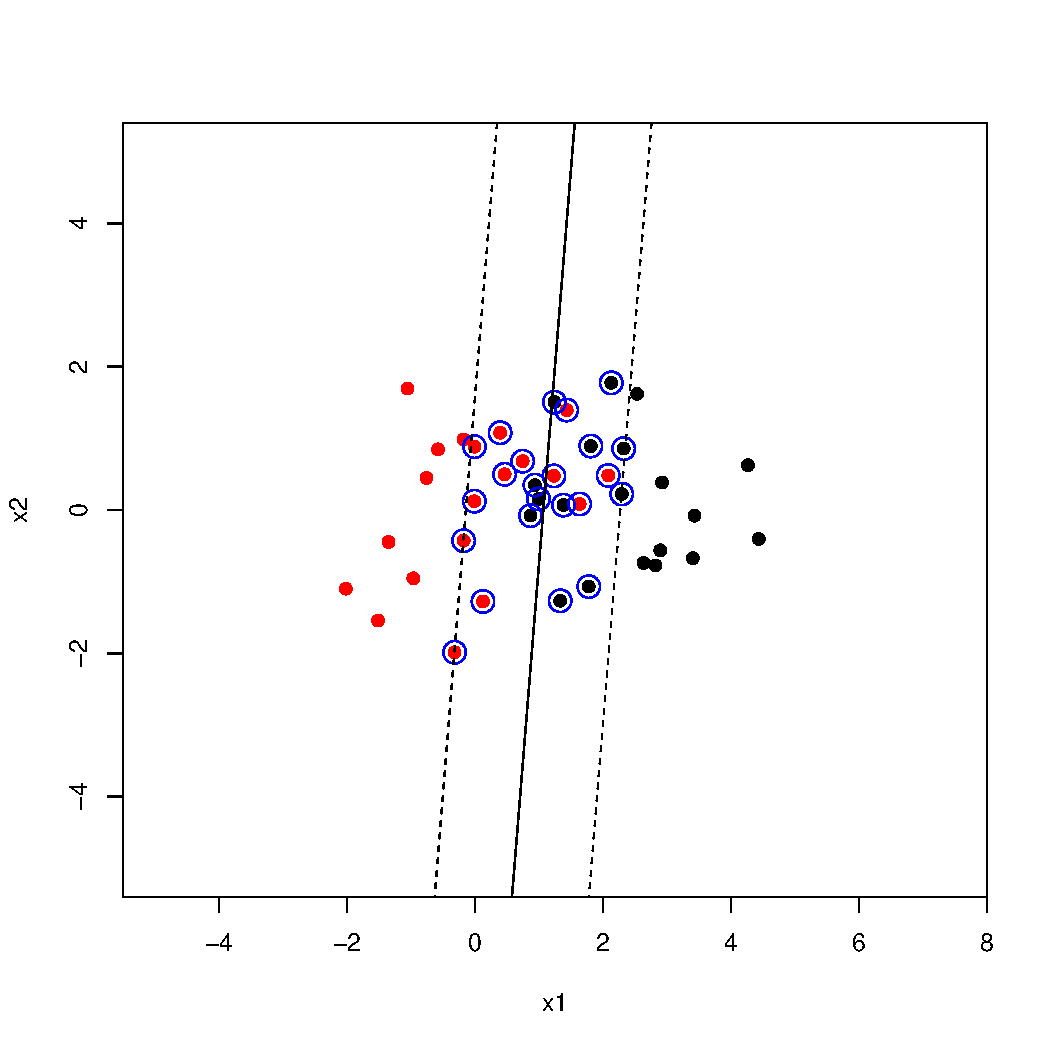
\includegraphics[width=0.5\textwidth]{plot1em2.pdf}%
	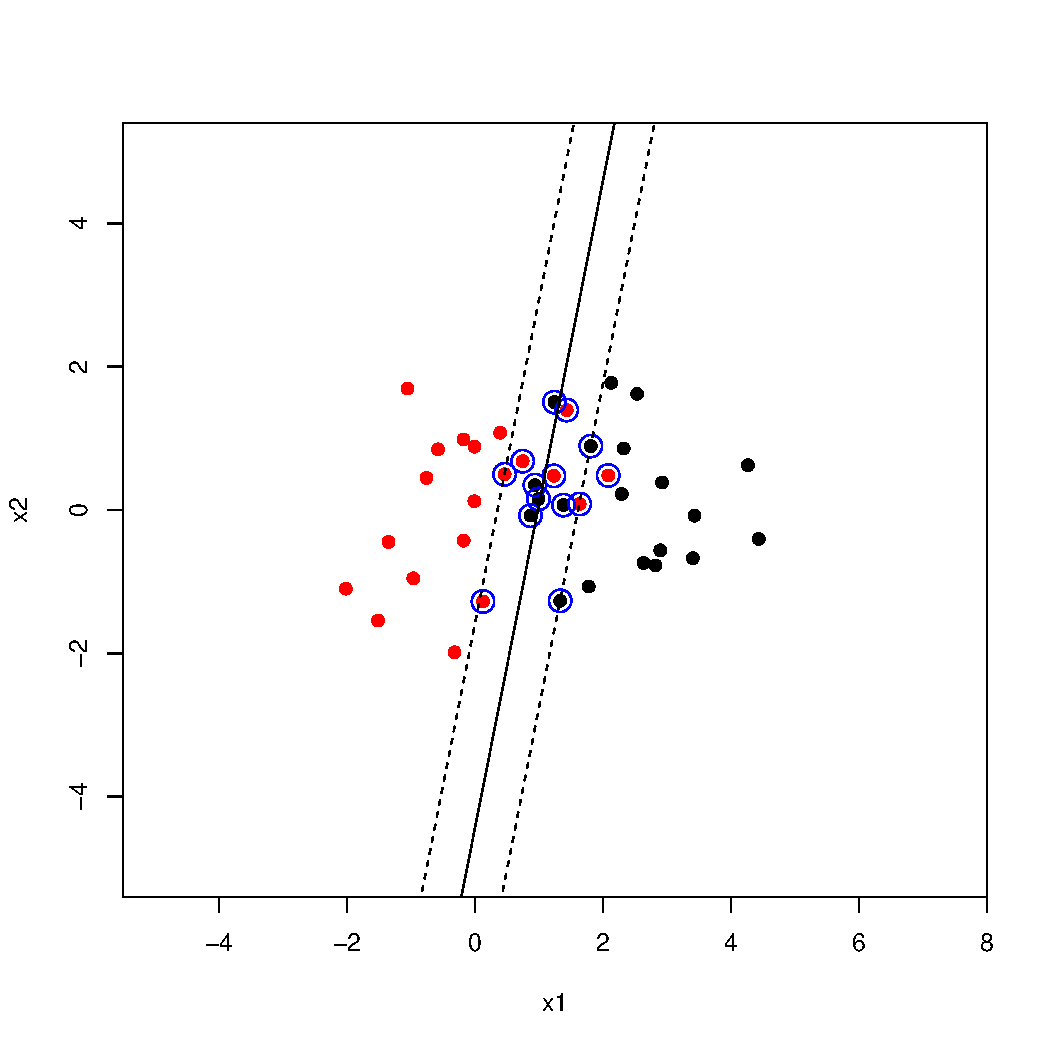
\includegraphics[width=0.5\textwidth]{plot1ep2.pdf}
	\caption{Влияние максимально допустимой ошибки на soft-margin SVM\label{fig:sm}}
\end{figure}

Параметр $t$, определяющий допустимое нарушение ограничений, позволяет варьировать количество опорных векторов (которые, вследствие KKT-условий,
соответствуют векторам, участвующим в построении классифицирующего правила; пример изменения
разделяющей гиперплоскости и набора опорных векторов показан на рисунке \ref{fig:sm}).

\subsection{Методы оптимизации}
В зависимости от соотношения размерностей $n$ и $p$, может быть выгодно (с точки зрения вычислительных затрат) решать прямую \eqref{eq:soft-primal},
или двойственную \ref{eq:soft-final} задачу.

При этом, несмотря на то, что обе задачи являются задачами квадратичного программирования с линейными
ограничениями неравенства, использование методов общего вида осложняется экспоненциальной (в худшем случае)
сложностью.

Для формулировки прямой задачи в виде 
	$$
		\sum\limits_{i=1}^n\max\left\{0, 1-y_i\left(x_i^\intercal \beta - \beta_0\right)\right\}+\eta\norm{\beta}^2_2\rightarrow \min\limits_{\beta,\beta_0}
		$$
предлагается использовать (стохастический) градиентный спуск со специфическим (для задачи SVM) выбором
величины шага (Pegasos: primal estimated sub-gradient solver for SVM); в этом случае можно показать,
что решение с точностью $\varepsilon$ достигается за $O\left(\frac{1}{\varepsilon}\right)$ итераций;
при этом количество наблюдений не влияет на асимптотику количества итераций.

Для двойственной задачи
	$$
		\mathcal{F}\left(\alpha_1,\dots,\alpha_n\right) = \sum\limits_{i=1}^{n}\alpha_i - \frac{1}{2}\sum\limits_{i=1}^n\sum\limits_{j=1}^n\alpha_i\alpha_jy_iy_jx_i^\intercal x_j \rightarrow \max\limits_{\alpha_i}
	$$
предлагается (A Dual Coordinate Descent Method for Large-scale Linear SVM) использовать покоординатный градиентный спуск:
	\begin{itemize}
		\item Каждый $\alpha_i$ изменяется в направлении $\frac{\partial \mathcal{F}}{\partial \alpha_i}$
		\item Очередное решение проецируется на множество допустимых
		\item Поддерживается необходимая для вычисления $x^\intercal \beta$ информация
	\end{itemize}

	Последовательность решений сходится как минимум линейно

\subsection{SVM как частный случай Empirical Risk Minimization}
Можно доказать, что задача SVM эквивалентна задаче 
\[
	C\sum\limits_{i=1}^{n}\max\left\{1-\left(x^\intercal\beta+\beta_0\right)y_i,0\right\}+\frac{1}{2}\norm{\beta}_2^2\rightarrow\min\limits_{\beta_0,\beta}
\]
где $C$ -- параметр алгоритма; домножив на $\frac{1}{nC}$ получается эквивалентная задача
\[
	\frac{1}{n}\sum\limits_{i=1}^{n}\max\left\{1-\left(x^\intercal\beta+\beta_0\right)y_i,0\right\}+\frac{t}{2}\norm{\beta}_2^2\rightarrow\min\limits_{\beta_0,\beta}
\]

В такой формулировке можно сравнить SVM, логистическую регрессию и LDA как непрерывные (SVM) и гладкие (LDA, логистическая регрессия)
аппроксимации ошибки классификации (в смысле методов минимизации [регуляризованного] эмпирического риска) следующими функциями потерь (графики функций
потерь приведены на рисунке \ref{fig:erm}):
\begin{itemize}
	\item SVM (hinge loss): $\max\left\{1-\left(x^\intercal\beta+\beta_0\right)y_i, 0\right\}$
	\item LDA%
		\footnote{В случае $\sum y_i=0$ можно показать следующую цепочку эквивалентных переходов: LDA $\Leftrightarrow$ FDA $\Leftrightarrow$ CCA (с 1 переменной в одном из наборов признаков) $\Leftrightarrow$ OLS $\sum\left(y_i-\left(\beta_0+\beta^\intercal x_i\right)\right)^2\rightarrow\min_{\beta,\beta_0}\Leftrightarrow ERM$}:
		$\left(1-y_i\left(\beta_0+\beta^\intercal x_i\right)\right)^2$
	\item Logistic regression: $\log\left(1+e^{-y_i\left(\beta^\intercal x_i+\beta_0\right)}\right)$
\end{itemize}

\begin{figure}
	\centering
	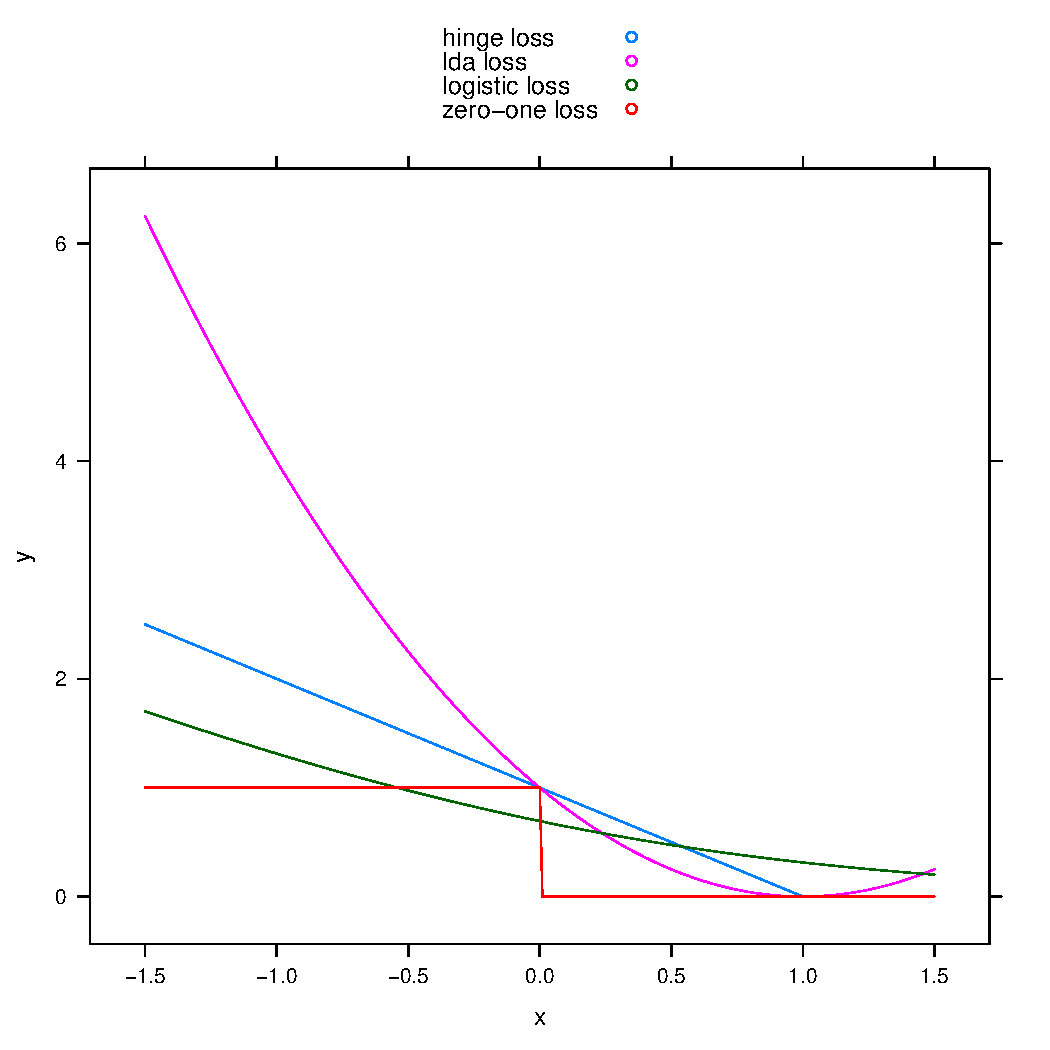
\includegraphics[width=0.8\textwidth]{loss.pdf}
	\caption{Различные функции потерь как непрерывные аппроксимации ошибки классификации\label{fig:erm}}
\end{figure}

Можно заметить, что LDA и логистическая регрессия имеют штраф и за правильно классифицированные наблюдения;
для логистической регрессии этот штраф убывает при удалении от разделяющей гиперплоскости, а для LDA ---
начинает увеличиваться при удалении от центра класса.

\section{Расширения SVM}
\subsection{Kernel trick\label{sec:KT}}
Описаный выше алгоритм может быть использован лишь в случае, когда данные относительно похожи на линейно-разделимые.

Предположим, что существует некоторое отображение $\Phi:\mathbb{R}^p\rightarrow V$ где $V$ -- некоторое гильбертово пространство.

Тогда, несложно заметить, что применяя SVM к образам исходных векторов, мы получаем задачу квадратичного программирования:
\begin{equation*}
\begin{cases}
\sum\limits_{i=1}^n\alpha_i-\frac{1}{2}\sum\limits_{i=1}^{n}\sum\limits_{k=1}^{n}\alpha_i\alpha_ky_iy_k\left\langle\Phi\left(x_i\right),\Phi\left(x_k\right)\right\rangle_V \rightarrow \max\limits_{\alpha_1,\dots,\alpha_n} \\
0 \leq \alpha_i \leq t, \forall i \\
\sum\limits_{i=1}^{n}\alpha_i y_i=0 \\
\end{cases}
\end{equation*}
и классифицирующая функция
\[
\begin{ecases}
h\left(x\right)=\sign\left[ \sum\limits_{i=1}^{n}\alpha_i y_i \left\langle \Phi\left(x_i\right), \Phi\left(x\right)\right\rangle_V - \beta_0\right]
\end{ecases}
\]
(правило классификации остаётся прежним --- $\sign\left(h\left(x\right)\right)$

Можно заметить, что во всех выражениях результат применения $\Phi$ используется только для использования в скалярном произведении с
результатом применения $\Phi$ к другому вектору из $\mathbb{R}^p$, что позволяет
(используя теорему Мерсера) использовать произвольную симметричную положительно
определённую функцию $k\left(u, v\right):\mathbb{R}^p\times\mathbb{R}^p\rightarrow \mathbb{R}$ (ядро) в качестве скалярного произведения
в некотором векторном пространстве; в этом случае преобразование
$\Phi$ может соответствовать отображению, состоящему из собственных функций $k$:
\begin{equation}
\begin{ecases}
k\left(u, v\right)=\sum\limits_{i=1}^\infty \theta_j \varphi_k\left(u\right) \varphi_k\left(v\right) \\
\Phi\left(x\right)=\left[\varphi_1\left(x\right),\dots,\varphi_k\left(x\right),\dots,\right] \\
\end{ecases}
\label{eq:decomp}
\end{equation}

Данное соображение позволяет применять SVM к данным в достаточной степени линейно разделимым в некотором гильбертовом пространстве
(в том числе --- бесконечномерном); в том числе --- без предъявления в явном виде отображения из исходного пространства в данное.

Так как непосредственная проверка положительной определённости ядра представляет собой проблему, можно
воспользоваться следующими операциями, приводящими к получению новых ядер:
	\begin{itemize}
		\item Скалярное произведение в векторном пространстве
		\item Положительная константа
		\item Произведение ядер: $K\left(u,v\right)=K_1\left(u,v\right)K_2\left(u, v\right)$
		\item Произведение отображений: $K\left(u, v\right)=\varphi\left(u\right)\varphi\left(v\right), \varphi:x\rightarrow \mathbb{R}$
		\item Линейная комбинация с положительными коэффициентами: $K\left(u, v\right)=\alpha_1K_1\left(u,v\right)+\alpha_2K_2\left(u, v\right), \alpha_{1,2}>0$
		\item Композиция ядра и отображения: $K\left(u, v\right)=K_1\left(\varphi\left(u\right),\varphi\left(v\right)\right)$
		\item Степенной ряд: 
			$$f: \mathbb{R}\rightarrow\mathbb{R}$$
			сходящийся степенной ряд с положительными коэффициентами, тогда
			$$K\left(u, v\right)=f\left(K_1\left(u,v\right)\right)$$
			является ядром
	\end{itemize}

Часто используемые ядра:
\begin{itemize}
	\item RBF (radial basis functions): $k\left(u, v\right)=e^{-\gamma\norm{u-v}_2^2}$
	\item Полиномиальное (степеней $\leq d$: $k\left(u, v\right)=\left(\left\langle u, v\right\rangle + 1\right)^d$
\end{itemize}

Используя \eqref{eq:decomp} можно показать, что использование полиномиального ядра степени $d$ соответствует
отображению в $C_{p+d}^{d}$-мерное пространство, гиперплоскостям в котором будут соответствовать поверхности
порядка $d$ в исходном пространстве.

Рассматривая RBF-ядро, можно убедиться, что $k\left(u,v\right)\xrightarrow[\gamma\rightarrow\infty]{}\mathbf{1}_{u=v}$;
что позволяет добиться линейной разделимости для произвольного набора данных (предполагая отсутствие наблюдений
с одинаковыми значениями признаков, принадлежащим разным классам).


\subsection{Изменение регуляризации}
	С целью отбора признаков можно изменить регуляризацию в одной из
	эквивалентных формулировок SVM:

	$$
		C\sum\limits_{i=1}^n\max\left\{0, 1-y_i\left(x_i^\intercal \beta - \beta_0\right)\right\}+\Phi\left(\beta\right)\rightarrow \min\limits_{\beta,\beta_0}
	$$

	\begin{itemize}
		\item LASSO SVM: $\Phi\left(\beta\right)=\norm{\beta}_1$
			\begin{itemize}
				\item Чем меньше $C$, тем больше влияние $\ell_1$-регуляризации
				\item Может попеременно отбрасывать и шумовые и значимые признаки при варьировании $C$
				\item Зависимые признаки не группируются
			\end{itemize}
		\item Doubly-regularized SVM: $\Phi\left(\beta\right)=\alpha\norm{\beta}_1+\frac{1}{2}\norm{\beta}_2^2$
			\begin{itemize}
				\item Чем больше $\alpha$, тем больше влияние $\ell_1$-регуляризации
				\item Присутствует эффект группировки
				\item Может попеременно отбрасывать и шумовые и значимые признаки при варьировании $C$, $\alpha$
			\end{itemize}
		\item Support Features Machine: $\Phi\left(\beta\right)=\sum\limits_{i=1}^{p}\max\left\{2\mu\beta_i, \mu^2+\beta_i^2\right\}$
			\begin{itemize}
				\item $\mu$ -- параметр <<селективности>>
				\item Присутствует эффект группировки
				\item Значимые ($\norm{\beta_j}>\mu$) признаки группируются и входят в решение совместно
				\item Шумовые признаки ($\norm{\beta_j}<\mu$) подавляются
			\end{itemize}
		\item Relevance Features Machine: $\Phi\left(\beta\right)=\sum\limits_{i=1}^{p}\ln\left(\beta_i^2+\frac{1}{\mu}\right)$
			\begin{itemize}
				\item $\mu$ -- параметр <<селективности>>
				\item Присутствует эффект группировки
			    \item Лучше выбирает набор значимых признаков	
			\end{itemize}
	\end{itemize}

    ($\alpha, \mu$ --- дополнительные параметры; коэффициент soft-margin SVM $t$, эквивалентным преобразованием перемещён к $\sum$)

\subsection{Support Vector Regression}
В секциях \ref{sec:hm}-\ref{sec:sm} было показано, что классифицирующее правило в SVM зависит только
от <<сложно>>-классифицируемых наблюдений (опорных векторов).

Оказывается, такую же идею можно использовать и для задач регрессии:
\[
\begin{cases}
\frac{1}{2}\beta^\intercal\beta\rightarrow\min\limits_{\beta,\beta_0}\\
\left\lvert y_i-\left(x_i^\intercal\beta+\beta_0\right)\right\rvert\leq\varepsilon\\
\end{cases}
\]
(где $\varepsilon$ -- параметр алгоритма); добавляя возможность нарушения ограничений,
переходим к задаче
\[
\begin{cases}
\frac{1}{2}\beta^\intercal\beta + C\sum\limits_{i=1}^n\left(\xi_i^++\xi_i^-\right)\rightarrow\min\limits_{\beta,\beta_0}\\
y_i-\left(x_i^\intercal\beta+\beta_0\right)\leq \varepsilon + \xi_i^+ \\
-y_i+\left(x_i^\intercal\beta+\beta_0\right)\leq \varepsilon + \xi_i^- \\
\xi_i^+\geq 0 \\
\xi_i^-\geq 0 \\
\end{cases}
\]

Можно показать, что двойственной к ней является задача
\[
\begin{cases}
\frac{1}{2}\sum\limits_{i=1}^n\sum\limits_{j=1}^n\left(\alpha_i^+-\alpha_i^-\right)\left(\alpha_j^+-\alpha_j^-\right)x_i^\intercal x_j+\varepsilon\sum\limits_{i=1}^n\left(\alpha_i^++\alpha_i^-\right)+\sum\limits_{i=1}^ny_i\left(\alpha_i^--\alpha_i^+\right)\rightarrow\min \\
\sum\limits_{i=1}^n\left(\alpha_i^+-\alpha_i^-\right)=0\\
0\leq\alpha_i^+\leq C \\
0\leq\alpha_i^-\leq C \\
\beta=\sum\limits_{i=1}^n\left(\alpha_i^+-\alpha_i^-\right)x_i \\
\end{cases}
\]

При этом, в силу KKT-условий, многие $\alpha_i=0$, т.е. в построении функции регрессии как и в SVM участвует
лишь ограниченное количество опорных наблюдений.

Аналогично SVM, двойственная задача регрессии допускает нелинейное обобщение с использованием kernel trick.

\subsection{Multi-class SVM}
В предъявленом построении SVM рассматривался лишь случай классификации с двумя классами.

Для распространения идеи SVM на классификацию с большим количеством классов существует несколько подходов, в частности:
\begin{itemize}
	\item Классификация с использованием сравнений вида ``один со многими''
	\item Классификация с использованием сравнений вида ``каждый с каждым''
\end{itemize}

\subsubsection{Сравнения ``один со многими''}
Для классификации с $N$ классами строится $N$ классифицирующих правил $h_i\left(x\right)$; кодирующих принадлежность $i$-му классу за $1$, 
а принадлежность любому другому классу за $-1$.

В качестве результирующего решающего правила используется
\[
h\left(x\right)=\argmax\limits_i h_i\left(x\right)
\]

\subsubsection{Сравнения ``каждый с каждым''}
Для классификации с $N$ классами строится $\frac{N\left(N-1\right)}{2}$ классифицирующих правил, производящих классификацию
для каждой возможной пары классов.

Обозначив за $N_i$ количество сравнений, в которых элемент $x$ был классифицирован как принадлежащий $i$-ому классу; в качестве
классифицирующего правила предлагается использовать 
\[
h\left(x\right)=\argmax\limits_i N_i
\]



\section{Выбор параметров}
Ввиду наличия свободы выбора значения параметра регуляризации, ядра (или семейства ядер), необходимо
предъявить процедуру сравнения построенных классификаторов. Так как в предлагаемой процедуре не используются
никакие предположения о распределении $P(x, y)$, использование информационных критериев (BIC, AIC, \dots) для
этих целей невозможно.

Предлагается рассмотреть процедуры выбора параметров, основанные на (общей) идее кросс-валидации и специфичную
для SVM оценку эмпирического риска на основе комбинаторной размерности.

\subsection{Кросс-валидация}
Предполагая, что выборка является выборкой из распределения $\langle x_i, y_i\rangle\sim\mathcal{P}\left(x,y\right)$,
с точки зрения выбора параметров или типа алгоритма классификации (или регрессии), хотелось бы получать не только
выборочную оценку качества классификации (регрессии), но и оценку пригодности выбранного алгоритма в смысле
качества классификации (регрессии) на всём распределении $\mathcal{P}$, а не только конкретной выборки из него.

Для этого предлагается построить несколько моделей по различным подмножествам датасета, оценить для каждой из моделей
качество классификации (регрессии) по части датасета, не участвовавшей в оценке параметров, после чего получить оценку
математического ожидания качества классификации (регрессии).

Обозначив за $N=\left\{1,\dots,n\right\}$ множество индексов элементов выборки, выберем $K$ подмножеств (примерно одинакового размера)
$N_k\subset N$.

Построим $K$ классификаторов (функций регрессии) $f_k\left(x\right)=f\left(x, \hat{\theta}\left(N\setminus N_k\right)\right)$.

\subsubsection{Классификация}
Для каждой из них вычислим эмпирическую ошибку классификации
\[
    \hat{\varepsilon}_k = \frac{1}{\#N_k}\sum\limits_{i\in N_k}\mathbf{1}_{f_k\left(x_i\right)\neq y_i}
\]

Используя данную оценку, построим оценку ошибки классификации
\[
    \hat{\varepsilon} = \frac{1}{n}\sum\limits_{i=1}^{K}\#N_k\hat{\varepsilon}_k
\]

Также можно оценить <<разброс>> ошибки классификации как
\[
    \hat{\sigma}_\varepsilon = \sqrt{\frac{1}{K-1}\sum\limits_{i=1}^K\left(\hat{\varepsilon}_k-\hat{\varepsilon}\right)^2}
\]

\subsubsection{Регрессия}
Для каждой из построенных моделей вычислим ошибку регрессии
\[
    \hat{\varepsilon}_k = \frac{1}{\#N_k}\sum\limits_{i\in N_k}\left(f_k\left(x_i\right) - y_i\right)^2
\]

И используя данные оценки, построим оценку дисперсии остатка регрессии для семейства $f$:
\[
    \hat{\varepsilon}=\frac{1}{n}\sum\limits_{i=1}^K \#N_k\hat{\varepsilon}_k
\]

\subsubsection{Общие соображения}
Получив оценки $\hat{\varepsilon}$ для всех интересующих параметрических семейств классификаторов (функций регрессии), следует выбрать
семейство, для которого $\hat{\varepsilon}$ минимальна. После этого имеет смысл повторить оценку параметров,
используя все доступные данные.

Стоит отметить, что оценки $\hat{\varepsilon}$ обычно консервативны (хуже, чем производительность наилучшего
представителя семейства с параметрами, оцененными по всем данным).

Существует несколько подходов к разделению выборки для cross-validation:
\begin{itemize}
    \item K-fold cross-validation: набор индексов $N$ разбивается на $K$ примерно-равных дизъюнктных подмножества $N_k$
    \item Leave-one-out cross-validation: $N$-fold cross-validation; рассматривается набор $N_k$, соответствующий всем
        одноэлементным подмножествам $N$
\end{itemize}


\subsection{Оценка через комбинаторную размерность}
Рассмотрим некоторое параметрическое семейство классификаторов $f_\alpha:\mathbb{R}^p\rightarrow\left\{-1,1\right\}$;
$\alpha$ --- параметры классификатора.

Предполагая, что выборка является выборкой из распределения $\langle x_i, y_i\rangle\sim\mathcal{P}\left(x,y\right)$
можно определить риск как
\[
R\left(\alpha\right)=\int\mathbf{1}_{y\neq f_\alpha\left(x\right)}\dd{\mathcal{P}\left(x, y\right)}
\]

Определив эмпирический риск (являющийся случайной величиной) как
\[
R_{emp}\left(\alpha\right)=\frac{1}{n}\sum\limits_{i=1}^n\mathbf{1}_{y_i\neq f_\alpha\left(x_i\right)}
\]
можно показать, что (независимо от $\mathcal{P})$ с вероятностью $1-\eta$ выполнено неравенство:

	$$	R\left(\alpha\right) \leq R_e\left(\alpha\right)+\sqrt{\frac{h\left(1+\log{\frac{2n}{h}}\right)-\log\frac{\eta}{4}}{n}}$$

где $h$ --- комбинаторная размерность семейства  классификаторов, определяемая как максимальное количество точек,
которые при любом их расположении и разделении на классы при некотором $\alpha$ будут безошибочно классифицированны.

Наример, для линейного классификатора в $p$-мерном пространстве VC-размерность составляет $p+1$,
для полиномиального ядра степени $d$ -- $C_{d+p}^{d}$ (ввиду числа мономов, являющихся собственными функциями ядра), для RBF VC-размерность бесконечна (см. описанную в \ref{sec:KT} конструкцию, разделяющую
произвольное множество точек на основе RBF).

Можно отметить, что при конечной $VC$-размерности и $n\rightarrow\infty$ дополнительное слагаемое стремится к $0$, т.е. $R_{emp}\left(\alpha\right)\rightarrow R\left(\alpha\right)$ по вероятности
(и эта сходимость наблюдается вне зависимости от конкретного распределения $\mathcal{P}$).

\end{document}
